\documentclass{AeroStructure-ERJohnson}
\input crosslink.tex

%\usepackage{showframe}
\def\ShowFrameLinethickness{0.125pt}

%\def\harp#1{\smash{\mathord{\buildrel{\lower3pt\hbox{$\scriptscriptstyle\rightharpoonup$}}\over{#1}}}}

\myexternaldocument{App_4P}
\myexternaldocument{Ch01_4P}
\myexternaldocument{Ch02_4P}
\myexternaldocument{Ch03_4P}
\myexternaldocument{Ch04_4P}
\myexternaldocument{Ch05_4P}
\myexternaldocument{Ch06_4P}
\myexternaldocument{Ch07_4P}
\myexternaldocument{Ch08_4P}
%\myexternaldocument{Ch09_4P}
\myexternaldocument{Ch10_4P}
\myexternaldocument{Ch11_4P}
\myexternaldocument{Ch12_4P}
\myexternaldocument{Ch13_4P}
\myexternaldocument{Ch14_4P}
\myexternaldocument{Ch15_4P}
\myexternaldocument{Ch16_4P}
\myexternaldocument{Ch17_4P}
\myexternaldocument{Ch18_4P}

\begin{document}

\mainmatter

\setcounter{page}{247}
\setcounter{chapter}{8}

\chapter[Failure initiation in FRP composites]{Failure initiation\break in FRP composites} \label{ch9}

\section{Strength of a composite ply} \label{sec9.1}

The strength of a laminated composite wall is assessed on a ply-by-ply basis. The main failure modes of unidirectional plies of fiber-reinforced polymer (FRP) composites are
\begin{itemize}
\item matrix compression failure,
\item matrix tension failure,
\item fiber compression failure,
\item fiber tension failure,
\item delamination.
\end{itemize}
The fiber modes and the matrix modes are intralaminar failure modes, meaning these failures occur within a ply. Intralaminar modes include fractures of the fiber and/or matrix, and fiber kinking or buckling in compression. Delamination is an interlaminar failure mode, and it refers to the formation of an interfacial crack, or a debonding, occurring between adjacent lamina with different fiber orientations. Delamination has been modeled with the concepts of fracture mechanics, where the displacements are discontinuous across the interfacial crack faces. An initial delamination crack is postulated and fracture mechanics principles are used to determine if the crack will propagate in a self-similar manner. Analysis of delamination by fracture mechanics is presented in article~\ref{sec13.7} on page~\pageref{sec13.7}.

Simple tests are conducted on unidirectional plies of FRP composites to determine its intralaminar failure strengths. There are five independent strengths of a unidirectional ply. Denote $X_{{T}}$ as the longitudinal tensile strength along the fiber direction, $X_{{C}}$ the longitudinal compression strength along the fiber direction, $Y_{{T}}$ the transverse tensile strength perpendicular to the fibers, $Y_{{C}}$ the transverse compression strength perpendicular to the fibers, and $S_{{L}}$ the longitudinal shear strength in the $x_1${-}$x_2$ plane. Typical values of the five basic strengths of selected composite materials are listed in table~\ref{tab9.1}.

\begin{table}
\processtable{Strengths of selected composite materials in MPa from Tsai (1992 p. 8-2) \label{tab9.1}}{
\begin{tabular}{@{}llll|lllll@{}}
\hline
%\toprule\\[-15pt]
%& & & & & & & & \\[-6pt]
& & & & & & & & \\[-5pt]
\multicolumn{4}{@{}l}{\colhead{Test and strength data}} & \multicolumn{5}{@{\hspace*{-0.25pt}}|l}{\colhead{Composite ply}} \\%[-5pt]
%\multicolumn{4}{@{}l}{\hrulefill} & \multicolumn{5}{@{}l@{}}{\hrulefill} \\
& & & & & & & & \\[-9pt]
\hline
& & & & & & & & \\[-9pt]
&  &  & & \colhead{T300/} &  & \colhead{E-glass/} & \colhead{Kevlar 49/} & \colhead{IM6/} \\
\colhead{Loading} & \colhead{Specimen} & \colhead{Strength MPa} & & \colhead{5208} & \colhead{AS/3501} & \colhead{epoxy} & \colhead{epoxy} & \colhead{epoxy} \\
%& & & & & & & & \\[-8pt]
%\midrule\\[-15pt]
% & & & & & & & & \\[-5pt]
& & & & & & & & \\[-9pt]
\hline
& & & & & & & & \\[-7pt]
Uniaxial & [0] & Longit tension & $X_{T}$ & 1{,}500 & 1{,}447 & 1{,}062 & 1{,}400 & 3{,}500 \\
Uniaxial & [0] & Longit compr & $X_{C}$ & 1{,}500 & 1{,}447 & \phantom{0,}610 & \phantom{0,}235 & 1{,}540\\
Uniaxial & [90] &Trans tension & $Y_{T}$ & \phantom{0,0}40& \phantom{0,0}52& \phantom{0,0}31& \phantom{0,0}12& \phantom{0,0}56\\
Uniaxial & [90]& Trans compr & $Y_{C}$& \phantom{0,}246& \phantom{0,}206& \phantom{0,}118& \phantom{0,0}53& \phantom{0,}150\\
Shear & [0] or [90]& Longit shear & $S_{L}$& \phantom{0,0}68 &\phantom{0,0}93& \phantom{0,0}72& \phantom{0,0}34& \phantom{0,0}98\\[-7pt]
& & & & & & & & \\[-4pt]
\botrule
\end{tabular}}{}
\vspace*{-1pc}
\end{table}

Failure criteria for unidirectional FRP composites based on general states of stress $\sigma_{11}$, $\sigma_{22}$, and $\sigma_{12}$ are reviewed in Tsai (1992, Section~8) and in Herakovich (1998, Section~9.3). Several of these criteria are in the form of dimensionless quadratic equations in the stress components with the five basic strengths appearing as parameters. The reader is referred to these references and the other references cited therein to see the details of these criteria. In the next subsection we review a recent criterion based on observed damage states.

\subsection{Puck's failure criterion}\label{sec9.1.1}

Intralaminar criteria for failure initiation have recently been assessed for FRP composites in the World-Wide Failure Exercise (WWFE) as summarized by Soden, et~al. (2004). Nineteen theoretical approaches for predicting the deformation and failure response of FRP composite laminates were compared to test results. At the conclusion of the WWFE five leading theories were selected to create recommendations and guidelines for designers. The theory proposed by Puck, et~al. (2002) was cited as one of the five producing the highest number of accurate predictions and capturing more general features of the experimental results. Puck's methodology assumes brittle fracture of polymer matrix composites, and distinguishes between fiber failure and inter-fiber failure (IFF) by separate criteria. Inter-fiber failure refers to cracks running parallel to the fibers through the thickness of a ply, with the plane of crack determined by three matrix-mode criteria denoted by A, B, and C.

With respect to the material principal directions $x_1$-$x_2$-$x_3$, the fracture plane is parallel to the $x_1$-axis as shown in figure~\ref{fig9.1}. Coordinates with respect to the fracture plane are denoted by $x_1$-$x_{n}$-$x_{t}$ with the $x_n$-axis normal to the plane. The $x_n$-axis is located by a counterclockwise rotation through the angle $\alpha$ about the $x_1$-axis. The relation between coordinate directions shown in figure~\ref{fig9.1} is given by the direction cosines of the angle~$\alpha$:
\begin{align}\label{eq9.1}
\left[\begin{array}{@{}l@{}}x_{1} \\x_{2} \\x_{3}\end{array}\right]=\left[\begin{array}{@{}ccc@{}}1 & 0 & 0 \\0 & \cos \alpha & -\sin \alpha \\0 & \sin \alpha & \cos \alpha\end{array}\right] \left[\begin{array}{@{}l@{}}x_{1} \\x_{n} \\x_{t}\end{array}\right], \textrm{ or } \left[\begin{array}{@{}l@{}}x_{1} \\x_{2} \\x_{3}\end{array}\right]=[\lambda]\left[\begin{array}{@{}l@{}}x_{1} \\x_{n} \\x_{t}\end{array}\right],
\end{align}
where $[\lambda]$ is the direction cosine matrix. The transformation from the stress components in the material principal directions to the stress components in the $x_1$-$x_{{n}}$-$x_{{t}}$ axis system is given eq. (\ref{eqA.96}) in the appendix. With due regard to the notation in this article this matrix transformation is
\begin{align}\label{eq9.2}
\left[\begin{array}{@{}lll@{}}\sigma_{11} & \sigma_{1 n} & \sigma_{1 t} \\\sigma_{n 1} & \sigma_{n n} & \sigma_{n t} \\\sigma_{t 1} & \sigma_{t n} & \sigma_{t t}\end{array}\right]=[\lambda]\left[\begin{array}{@{}lll@{}}\sigma_{11} & \sigma_{12} & \sigma_{13} \\\sigma_{12} & \sigma_{22} & \sigma_{23} \\\sigma_{13} & \sigma_{23} & \sigma_{33}\end{array}\right][\lambda]^{T}.
\end{align}
\vspace*{3pt}
\pagebreak

\noindent Complete the matrix multiplication in the previous equation to find the stress components $\sigma_\textit{nn}$, $\sigma_\textit{nt}$, and $\sigma_{n1}$ acting on the fracture plane in terms of the stress components in the principal material directions. The results are
\begin{align}\label{eq9.3}
\begin{gathered}\sigma_{n n}=\frac{1}{2}\left(\sigma_{22}+\sigma_{33}\right)+\frac{1}{2}\left(\sigma_{22}-\sigma_{33}\right) \cos 2 \alpha+\sigma_{23} \sin 2 \alpha \\\sigma_{n t}=-\frac{1}{2}\left(\sigma_{22}-\sigma_{33}\right) \sin 2 \alpha+\sigma_{23} \cos 2 \alpha. \\\sigma_{n 1}=\sigma_{21} \cos \alpha+\sigma_{31} \sin \alpha\end{gathered}
\end{align}
Note that the stress component $\sigma_\textit{11}$ does not appear in a criterion formulated from the stress components on the fracture plane.

\begin{figure}[!h]
\centerline{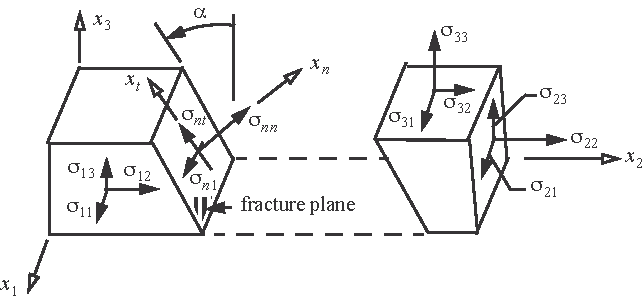
\includegraphics{Figure_9-1.pdf}}
\caption{Inter-fiber fracture plane is located by rotation through angle $\alpha$ about the $x_1$-axis. \label{fig9.1}}
\end{figure}

Puck's criteria are expressed in terms of a dimensionless failure index denoted by \textit{FI} for either a matrix mode \textit{FI}$_M$ or a fiber mode \textit{FI}$_F$. The range of the failure indices are $0 \leq F I<1$ for no failure, and $F I=1$ at failure initiation.


\subsubsection{Matrix mode A.}\quad In the uniaxial transverse tension test and the in-plane shear test, the plane of fracture is normal to the $x_2$-direction so $\alpha= 0$. From eq.~(\ref{eq9.3}) the stresses on the fracture plane are $\sigma_\textit{nn} = \sigma_\textit{22}$, $\sigma_\textit{nt} = \sigma_{23}$, and $\sigma_{n1} = \sigma_\textit{21}$.{\parfillskip=0pt\par}

\begin{wrapfigure}[11]{L}{113.25pt}
\vspace{-10pt}
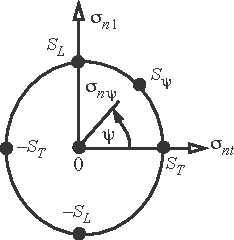
\includegraphics{Figure_9-2.pdf}
\caption{$\boldsymbol{\sigma}_{nn}= {\textbf{0}}$ plane. \label{fig9.2}}
\end{wrapfigure}

\vspace*{-1pc}

\noindent In the transverse tension test $\sigma_\textit{22} = Y_T$ at failure, and all other stresses in the $x_i$-system vanish. For the in-plane shear test all stresses in the $x_i$-system vanish except that $\sigma_\textit{21} = S_L$ at failure. The proposed criterion including these test results is quadratic and of the form
\begin{align}\label{eq9.4}
\left(1-c_{1}\right)\left(\frac{\sigma_{n n}}{Y_{T}}\right)^{2}+c_{1}\left(\frac{\sigma_{n n}}{Y_{T}}\right)+\left(\frac{\sigma_{n t}}{S_{T}}\right)^{2}+\left(\frac{\sigma_{n 1}}{S_{L}}\right)^{2}=1 \quad \sigma_{n n} \geq 0.
\end{align}

\vspace*{-1pc}

\noindent The shear strength transverse to the fibers in the fracture plane is denoted by $S_T$ in eq.~(\ref{eq9.4})\footnote{There is no simple test to determine $S_T$ for FRP composites. In Puck's criterion $S_T$ is determined from the pure transverse compression test. Refer to eq. (\ref{eq9.49}) on page~\pageref{eq9.49}.}. In the Cartesian coordinates with axes $\sigma_\textit{nn}$, $\sigma_\textit{nt}$, and $\sigma_{n1}$ the surface given by eq.~(\ref{eq9.4}) is an ellipsoid if the constant $c_1 < 1$. In the shear stress plane $\sigma_\textit{nt}$-$\sigma_{n1}$ where $\sigma_\textit{nn}$ is equal to zero, the cross section of the ellipsoid is an ellipse shown in figure~\ref{fig9.2}. The equation for the ellipse in the plane $\sigma_\textit{nn}$ equal to zero is
\begin{align}\label{eq9.5}
\left(\frac{\sigma_{n t}}{S_{T}}\right)^{2}+\left(\frac{\sigma_{n 1}}{S_{L}}\right)^{2}=1 \quad \sigma_{n n}=0.
\end{align}
The resultant of the shear stress components is denoted by $\sigma_{n\psi}$, and the angle between the line of action of the resultant and $\sigma_\textit{nt}$-axis is denoted by $\psi$. The stress components are related to the resultant by
\begin{align}\label{eq9.6}
\sigma_{n t}=\sigma_{n\psi} \cos \psi \quad \sigma_{n 1}=\sigma_{n \psi} \sin \psi.
\end{align}
Substitute eq.~(\ref{eq9.6}) for the stress components in eq.~(\ref{eq9.5}) to get
\begin{align}\label{eq9.7}
\sigma_{n \psi}^{2}\left(\frac{\cos ^{2}{\kern-1pt\psi}}{S_{T}^{2}}+\frac{\sin ^{2}{\kern-1pt\psi}}{S_{L}^{2}}\right)=1 \quad \sigma_{n n}=0.
\end{align}
On the failure ellipse $\sigma_{n \psi}=S_{\psi}$ in eq.~(\ref{eq9.7}). Hence, strength $S_{\psi}$ is related to strengths $S_T$ and  $S_L$ by
\begin{align}\label{eq9.8}
S_{\psi}^{2}\left(\frac{\cos ^{2}{\kern-1pt\psi}}{S_{T}^{2}}+\frac{\sin ^{2}{\kern-1pt\psi}}{S_{L}^{2}}\right)=1 \quad \sigma_{n n}=0.
\end{align}

To interpret constant $c_1$ we take the differential of (\ref{eq9.4}) with respect to $\sigma_\textit{nn}$ followed by setting $\sigma_\textit{nn} = 0$ to get
\begin{align}\label{eq9.9}
\frac{c_{1}}{Y_{T}}+\frac{2 \sigma_{n t}}{S_{T}^{2}} \frac{d \dot{\sigma}_{n t}}{d \sigma_{n n}}+\frac{2 \sigma_{n 1}}{S_{L}^{2}} \frac{d \sigma_{n 1}}{d \sigma_{n n}}=0 \quad \sigma_{n n}=0.
\end{align}
Along the curve on the ellipsoid defined by angle $\psi$ equal to a constant, substitute the relations (\ref{eq9.6}) with $\sigma_{n \psi}=S_{\psi}$ into eq.~(\ref{eq9.9}) to get
\begin{align}\label{eq9.10}
\frac{c_{1}}{2 Y_{T}}+S_{\psi}\left(\frac{\cos ^{2}{\kern-1pt\psi}}{S_{T}^{2}}+\frac{\sin ^{2}{\kern-1pt\psi}}{S_{L}^{2}}\right) \frac{d \sigma_{n \psi}}{d \sigma_{n n}}=0 \quad \sigma_{n n}=0.
\end{align}
Use the result in eq.~(\ref{eq9.8}) to write eq.~(\ref{eq9.10}) as
\begin{align}\label{eq9.11}
\frac{c_{1}}{2 Y_{T}}+\frac{1}{S_{\psi}} \frac{d \sigma_{n \psi}}{d \sigma_{n n}}=0 \quad \sigma_{n n}=0.
\end{align}
Along the curve on the ellipsoid defined by angle $\psi$ equal to a constant, let the negative of the slope of the $\sigma_{n \psi}$ with respect to $\sigma_\textit{nn}$ at $\sigma_\textit{nn} = 0$ be denoted by $p_{n\psi}^{(+)}$. That is,
\begin{align}\label{eq9.12}
p_{n \psi}^{(+)}=-\left.\frac{d \sigma_{n \psi}}{d \sigma_{n n}}\right|_{\sigma_{n n}=0}.
\end{align}
Puck defines $p_{n \psi}^{(+)}$ as an inclination parameter. Therefore, the constant $c_1$ is determined from
\begin{align}\label{eq9.13}
\frac{c_{1}}{2 Y_{T}}=\frac{p_{n \psi}^{(+)}}{S_{\psi}}.
\end{align}
Substitute the constant $c_1$ determined from eq.~(\ref{eq9.13}) into eq.~(\ref{eq9.4}) to get the failure criterion for mode A as
\begin{align}\label{eq9.14}
\left(1-\frac{2 Y_{T}}{S_{\psi}} p_{n \psi}^{(+)}\right)\left(\frac{\sigma_{n n}}{Y_{T}}\right)^{2}+\frac{2 Y_{T}}{S_{\psi}} p_{n \psi}^{(+)}\left(\frac{\sigma_{n n}}{Y_{T}}\right)+\left(\frac{\sigma_{n t}}{S_{T}}\right)^{2}+\left(\frac{\sigma_{n 1}}{S_{L}}\right)^{2}=1 \quad \sigma_{n n} \geq 0.
\end{align}
The following failure index for mode A is given by Puck:
\begin{align}\label{eq9.15}
F I_{M}=\sqrt{\left[1-\frac{Y_{T}}{S_{\psi}} p_{n \psi}^{(+)}\right]^{2}\left(\frac{\sigma_{n n}}{Y_{T}}\right)^{2}+\left(\frac{\sigma_{n t}}{S_{T}}\right)^{2}+\left(\frac{\sigma_{n 1}}{S_{L}}\right)^{2}}+p_{n \psi}^{(+)}\left(\frac{\sigma_{n n}}{S_{\psi}}\right) \quad \sigma_{n n} \geq 0.
\end{align}
To show eqs. (\ref{eq9.14}) and (\ref{eq9.15}) are equivalent: Set $F I_{M}=1$ in (\ref{eq9.15}) and subtract $\frac{Y_{T}}{S_{\psi}} p_{n \psi}^{(+)}\left(\frac{\sigma_{n n}}{Y_{T}}\right)$ from each side. Then square the result to arrive at eq.~(\ref{eq9.14}) after some algebraic manipulations.

The inclination parameter $p_{n \psi}^{(+)}$ is related to the inclination parameters defined for the $\psi= 0$ and $\psi=\pi/2$ failure loci on the ellipsoid. The locus of failure initiation for $\psi=0$ is a curve in the $\sigma_\textit{nn}$-$\sigma_\textit{nt}$ plane. At the point on this curve where $\left(\sigma_{n n}, \sigma_{n 1}\right)=(0,0)$ failure initiates when $\sigma_{n t}=S_{T}=S_{\psi}$. The gradient condition at this point from eq.~(\ref{eq9.9}) is
\begin{align}\label{eq9.16}
\frac{c_{1}}{2 Y_{T}}+\frac{1}{S_{T}} \frac{d \dot{\sigma}_{n t}}{d \sigma_{n n}}=0.
\end{align}
The locus of failure initiation for $\psi=\pi/2$ is a curve in the $\sigma_\textit{nn}$-$\sigma_{n1}$ plane. At the point on this curve where $\left(\sigma_{n n}, \sigma_{n t}\right)=(0,0)$ failure initiates when $\sigma_{n 1}=S_{L}=S_{\psi}$. The gradient condition at this point from eq.~(\ref{eq9.9}) is
\begin{align}\label{eq9.17}
\frac{c_{1}}{2 Y_{T}}+\frac{1}{S_{L}} \frac{d \sigma_{n 1}}{d \sigma_{n n}}=0.
\end{align}
Define the inclination parameter on the $\psi=0$ curve as $p_{n t}^{(+)}=-\frac{d \dot{\sigma}_{n t}}{d \sigma_{n n}}$, and on the $\psi=\pi/2$ curve as $p_{n 1}^{(+)}=-\frac{d \sigma_{n 1}}{d \sigma_{n n}}$. Combine eqs. (\ref{eq9.13}), (\ref{eq9.16}), and (\ref{eq9.17}) to find
\begin{align}\label{eq9.18}
\frac{p_{n \psi}^{(+)}}{S_{\psi}}=\frac{p_{n t}^{(+)}}{S_{T}}, \textrm{ and } \frac{p_{n \psi}^{(+)}}{S_{\psi}}=\frac{p_{n 1}^{(+)}}{S_{L}}.
\end{align}
Multiply the first expression in eq.~(\ref{eq9.18}) by $\cos ^{2}{\kern-1pt\psi}$, and add it to the second expression in eq.~(\ref{eq9.18}) multiplied by $\sin ^{2}{\kern-1pt\psi}$, to get relationship between the inclination parameters on the tension side of the ellipse in figure~\ref{fig9.2} as
\begin{align}\label{eq9.19}
\frac{p_{n \psi}^{(+)}}{S_{\psi}}=\frac{p_{n t}^{(+)}}{S_{T}} \cos ^{2}{\kern-1pt\psi}+\frac{p_{n 1}^{(+)}}{S_{L}} \sin ^{2}{\kern-1pt\psi}.
\end{align}

\subsubsection{Matrix modes B and C.}\quad These modes are defined for a compressive normal stress, $\sigma_\textit{nn} < 0$, acting on the fracture plane. The motivation of Puck's criterion for modes B and C is the Coulomb-Mohr (C-M) criterion (Dowling, 1993, pp. 255--261) for failure of brittle materials. In the C-M criterion a compressive normal stress resists fracture caused by the shear stresses $\sigma_\textit{nt}$ and $\sigma_{n1}$. The C-M criterion can be considered to be a shear stress criterion in which the limiting shear stress increases for larger amounts of compression. Consider the case where $\sigma_{\textrm{n1}} = 0$, so on the fracture plane $\sigma_{\textrm{nn}} < 0$ and $\sigma_{n t}\neq 0$. Then the C-M criterion can be written in the form $\left|\sigma_{n t}\right|+\mu \sigma_{n n}=S_{T}$, where $\mu$ is a friction coefficient and $S_T$ is the shear strength transverse to the fibers in the fracture plane. The friction effect, $\mu \sigma_{n n}$, can be used to increase the strength or to decrease the applied shear stress in a C-M criterion. Puck and Sch\"{u}mann (1998) proposed the following criterion
\begin{align}\label{eq9.20}
\left(\frac{\sigma_{n t}}{S_{T}-p_{n t}^{(-)} \sigma_{n n}}\right)^{2}+\left(\frac{\sigma_{n 1}}{S_{L}-p_{n 1}^{(-)} \sigma_{n n}}\right)^{2}=1 \quad \sigma_{n n} \leq 0,
\end{align}
in which the strengths in the denominators are increased by the compressive normal stress, and $\left(p_{n t}^{(-)}, p_{n 1}^{(-)}\right)$ are the inclination parameters in compression. Set $\sigma_{n1} = 0$ in eq.~(\ref{eq9.20}) to get $\sigma_{n t}=S_{T}-p_{n t}^{(-)} \sigma_{nn}$, and from this expression the inclination parameter is interpreted as the negative slope of $\sigma_\textit{nt}$ with respect to $\sigma_\textit{nn}$, or
\begin{align}\label{eq9.21}
p_{n t}^{(-)}=-\left.\left(\frac{d \sigma_{n t}}{d \sigma_{n n}}\right)\right|_{\sigma_{n 1}=0}.
\end{align}
Set $\sigma_\textit{nt} = 0$ in eq.~(\ref{eq9.20}) to get $\sigma_{n 1}=S_{L}-p_{n}^{(-)} \sigma_{n n}$, and from this expression the inclination parameter is interpreted as the negative slope of $\sigma_{n1}$ with respect to $\sigma_\textit{nn}$, or
\begin{align}\label{eq9.22}
p_{n 1}^{(-)}=-\left.\left(\frac{d \sigma_{n 1}}{d \sigma_{n n}}\right)\right|_{\sigma_{n t}=0}.
\end{align}

Citing better agreement with experimental results, the denominators of the shear stresses in eq.~(\ref{eq9.20}) are expanded and the quadratic terms in the normal stress $\sigma_\textit{nn}$ are neglected with respect to the linear terms in $\sigma_\textit{nn}$, so the criterion reduces to
\begin{align}\label{eq9.23}
\frac{\sigma_{n t}^{2}}{S_{T}^{2}-2 p_{n t}^{(-)} S_{T} \sigma_{n n}}+\frac{\sigma_{n 1}^{2}}{S_{L}^{2}-2 p_{n 1}^{(-)} S_{L} \sigma_{n n}}=1 \quad \sigma_{n n} \leq 0.
\end{align}
For mathematical simplification Puck and Sh\"{u}mann assume that the inclination parameters are related in a similar way to eq.~(\ref{eq9.18}) by
\begin{align}\label{eq9.24}
\frac{p_{n t}^{(-)}}{S_{T}}=\frac{p_{n 1}^{(-)}}{S_{L}}=\frac{p}{R}.
\end{align}
With this assumption eq.~(\ref{eq9.23}) reduces to the simpler form
\begin{align}\label{eq9.25}
\left(\frac{\sigma_{n t}}{S_{T}}\right)^{2}+\left(\frac{\sigma_{n 1}}{S_{L}}\right)^{2}+2\left(\frac{p}{R}\right) \sigma_{n n}=1 \quad \sigma_{n n} \leq 0.
\end{align}
In the Cartesian coordinates with axes $\sigma_\textit{nn}$, $\sigma_\textit{nt}$, and $\sigma_{n1}$ the surface given by eq.~(\ref{eq9.25}) is an elliptic paraboloid. Note that the failure surface does not intersect the negative $\sigma_\textit{nn}$-axis according to the hypothesis that a compressive normal stress impedes a shear fracture (i.e., the shear resistance to fracture means the contour lines in the failure surface increase with increasing compression). In the shear stress plane $\sigma_\textit{nt}$-$\sigma_{n1}$ where $\sigma_\textit{nn}$ is equal to zero, the cross section of the ellipsoid is an ellipse shown in figure~\ref{fig9.2}. Substitute the relations given by eq.~(\ref{eq9.6}) into eq.~(\ref{eq9.25}) to get
\begin{align}\label{eq9.26}
\sigma_{n \psi}^{2}\left(\frac{\cos ^{2}{\kern-1pt\psi}}{S_{T}^{2}}+\frac{\sin ^{2}{\kern-1pt\psi}}{S_{L}^{2}}\right)+2\left(\frac{p}{R}\right) \sigma_{n n}=1 \quad \sigma_{n n} \leq 0.
\end{align}
Differentiate eq.~(\ref{eq9.26}) with respect to $\sigma_\textit{nn}$ to get
\begin{align}\label{eq9.27}
\sigma_{n \psi}\left(\frac{\cos ^{2}{\kern-1pt\psi}}{S_{T}^{2}}+\frac{\sin ^{2}{\kern-1pt\psi}}{S_{L}^{2}}\right) \frac{d \sigma_{n \psi}}{d \sigma_{n n}}+\frac{p}{R}=0.
\end{align}
Consider the $\sigma_\textit{nt}$-$\sigma_{n1}$ plane at $\sigma_\textit{nn}=0$. On the failure ellipse $\sigma_{n\psi}=S_{\psi}$ and (\ref{eq9.26}) is
\begin{align}\label{eq9.28}
S_{\psi}^{2}\left(\frac{\cos ^{2}{\kern-1pt\psi}}{S_{T}^{2}}+\frac{\sin ^{2}{\kern-1pt\psi}}{S_{L}^{2}}\right)=1.
\end{align}
Evaluate eq.~(\ref{eq9.27}) at $\sigma_{n \psi}=S_{\psi}$, followed by the substitution of eq.~(\ref{eq9.28}). The result is
\begin{align}\label{eq9.29}
\frac{1}{S_{\psi}} \frac{d \sigma_{n \psi}}{d \sigma_{n n}}+\frac{p}{R}=0 \quad \sigma_{n n}=0.
\end{align}
Define the inclination parameter for the curve $\psi$ equal to a constant by $p_{n\psi}^{(-)}=-\frac{d \sigma_{n \psi}}{d \sigma_{n n}}$. Hence,
\begin{align}\label{eq9.30}
\frac{p}{R}=\frac{p_{n \psi}^{(-)}}{S_{\psi}}.
\end{align}
Substitute the result (\ref{eq9.30}) into the condition of failure initiation (\ref{eq9.25}) to find
\begin{align}\label{eq9.31}
\left(\frac{\sigma_{n t}}{S_{T}}\right)^{2}+\left(\frac{\sigma_{n 1}}{S_{L}}\right)^{2}+2\left(\frac{p_{n \psi}^{(-)}}{S_{\psi}}\right) \sigma_{n n}=1 \quad \sigma_{n n} \leq 0.
\end{align}
The following failure index for $\sigma_{n n} \leq 0$ is given by Puck.
\begin{align}\label{eq9.32}
F I_{M}=\sqrt{\left(\frac{\sigma_{n t}}{S_{T}}\right)^{2}+\left(\frac{\sigma_{n 1}}{S_{L}}\right)^{2}+\left(\frac{p_{n \psi}^{-}}{S_{\psi}} \sigma_{n n}\right)^{2}}+\left(\frac{p_{n \psi}^{(-)}}{S_{\psi}}\right) \sigma_{n n} \quad \sigma_{n n} \leq 0.
\end{align}
One can show eq.~(\ref{eq9.32}) is equivalent to eq.~(\ref{eq9.31}) if we set $F I_{M}=1$ in (\ref{eq9.32}).

Combining eqs. (\ref{eq9.24}) and (\ref{eq9.30}) we get
\begin{align}\label{eq9.33}
\frac{p_{n \psi}^{(-)}}{S_{\psi}}=\frac{p_{n t}^{(-)}}{S_{T}}, \textrm{ and } \frac{p_{n \psi}^{(-)}}{S_{\psi}}=\frac{p_{n}^{(-)}}{S_{L}}
\end{align}
Similar to the manipulations to get eq.~(\ref{eq9.19}), the expressions in eq.~(\ref{eq9.33}) lead to the relationship between the inclination parameters on the compression side of the ellipse of figure~\ref{fig9.2} as
\begin{align}\label{eq9.34}
\frac{p_{n \psi}^{(-)}}{S_{\psi}}=\frac{p_{n t}^{(-)}}{S_{T}} \cos ^{2}{\kern-1pt\psi}+\frac{p_{n 1}^{(-)}}{S_{L}} \sin ^{2}{\kern-1pt\psi}.
\end{align}

\removelastskip

For given values of the stress components $\sigma_{22}$, $\sigma_{33}$, $\sigma_{23}$, $\sigma_{21}$, and $\sigma_{31}$ for which $\sigma_{n n} \leq 0$, the failure index is a function of the angle $\alpha$ of the fracture plane. The condition to find $\alpha$ is to make the failure index a maximum. The necessary condition for a maximum is $\frac{\partial F I_{M}}{\partial \alpha}=0$. To find $\alpha$ that satisfies the necessary condition requires a numerical search.

\looseness=-1{}The section of the failure surface in the $\sigma_\textit{nn}$-$\sigma_\textit{nt}$ plane where $\sigma_{n1} = 0$ is shown in figure~\ref{fig9.3}(a), and the section of the failure surface in the $\sigma_\textit{nn}$-$\sigma_{n1}$ plane where $\sigma_\textit{nt} = 0$ is shown in figure~\ref{fig9.3}(b). In addition to the five basic strength data for an FRP composite ply listed in table~\ref{tab9.1}, Puck's criterion introduces four new dimensionless parameters: $p_{n1}^{(+)}$, $p_{n t}^{(+)}$, $p_{n t}^{(-)}$, and $p_{n 1}^{(-)}$. The inclination parameters $p_{n t}^{(-)}$ and $p_{n t}^{(+)}$ are the slopes of the failure locus at the $\sigma_{nt}$-axis in figure~\ref{fig9.3}(a). Inclination parameters $p_{n1}^{(-)}$ and $p_{n 1}^{(+)}$ are the slopes of the failure locus at the $\sigma_{n1}$-axis shown in figure~\ref{fig9.3}(b). Puck, et~al. (2002) recommend that $p_{n t}^{(-)}=p_{n t}^{(+)}$, which makes the slope of the $\sigma_\textit{nn}$-$\sigma_\textit{nt}$ curve continuous at the $\sigma_\textit{nt}$-axis. The inclination parameters $p_{n 1}^{(-)}=0.25$ and $p_{n 1}^{(+)}=0.30$ with $p_{n t}^{(-)}$ computed from eq.~(\ref{eq9.24}) were used in the WWFE. Recommended ranges of inclination parameters are listed table~\ref{tab9.2}.

\processfigure[!h]{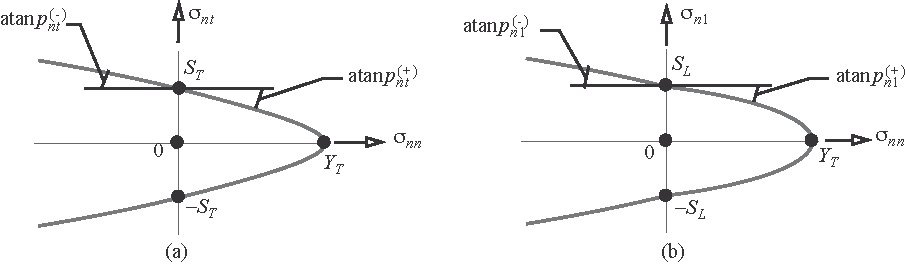
\includegraphics{Figure_9-3.pdf}}{\caption{(a) Sections of the failure surface in the $\sigma_{nn}$-$\sigma_{nt}$ plane, and (b) in the $\sigma_{nn}$-$\sigma_{n\textbf{1}}$ plane.}\label{fig9.3}}

\begin{table}[!h]
\processtable{Recommended range for inclination parameter $\textbf{\textit{p}}_{\textbf{\textit{nt}}}$ from Puck et~al. (2002) \label{tab9.2}}{
\tabcolsep=10pt\begin{tabular}{@{}lcc@{}}
\toprule
& \colhead{$p_{n t}^{(-)}$} & \colhead{$p_{n t}^{(+)}$} \\
\midrule
Glass-fiber/epoxy & 0.20 to 0.25 & 0.20 to 0.25\\
Carbon-fiber/epoxy & 0.25 to 0.30 & 0.25 to 0.30 \\
\botrule
\end{tabular}}{}
\vspace*{-1pc}
\end{table}


\subsubsection{Fiber modes.} A simple fiber mode criterion that does not interact with the longitudinal shear stresses $\sigma_{21}$ and $\sigma_{31}$ is the maximum stress criterion along the fibers. The fiber failure index $F I_{F}$ is defined by
\begin{align}\label{eq9.35}
F I_{F}= \begin{cases}\frac{-\sigma_{11}}{X_{c}} & \sigma_{11}<0 \\[5pt]
\frac{\sigma_{11}}{X_{T}} & \sigma_{11}>0\end{cases},
\end{align}
where $0 \leq F I_{F}<1$ for no failure of the fiber, and $F I_{F}=1$ at failure.

\subsection{Matrix failure criteria for a plane stress state}\label{sec9.1.2}

The assumption of plane stress is that out-of-plane stresses $\sigma_{33}$, $\sigma_{23}$, and $\sigma_{31}$ are negligible in comparison to the in-plane stress components $\sigma_{22}$ and $\sigma_{21}$. Hence, the out-of-plane stresses can be neglected in the stress transformation equations (\ref{eq9.3}). The stress transformation equations reduce to
\begin{align}\label{eq9.36}
\sigma_{nn}=\sigma_{22} \cos ^{2}\alpha \quad \sigma_{n t}=-\sigma_{22} \sin \alpha \cos \alpha \quad \sigma_{n 1}=\sigma_{21} \cos \alpha.
\end{align}

In \textbf{mode A} $\alpha= 0$, and stresses $\sigma_{\textit{nn}} = \sigma_{22}$, $\sigma_{\textit{nt}} = 0$, and $\sigma_{{n1}} = \sigma_{21}$. For $\sigma_{\textit{nt}} = 0$ the locus of failure initiation is a curve in the $\sigma_{\textit{nn}}$-$\sigma_{{n1}}$ plane and $\psi=\pi/2$. From eq.~(\ref{eq9.19}) we find $\frac{p_{n\psi}^{(+)}}{S_{\psi}}=\frac{p_{n 1}^{(+)}}{S_{L}}$. Therefore, the mode A failure index. (\ref{eq9.15}) in plane stress reduces to
\begin{align}\label{eq9.37}
F I_{M}=\sqrt{\left[1-p_{n 1}^{(+)} \frac{Y_{T}}{S_{L}}\right]^{2}\left(\frac{\sigma_{22}}{Y_{T}}\right)^{2}+\left(\frac{\sigma_{21}}{S_{L}}\right)^{2}}+\frac{p_{n 1}^{(+)} \sigma_{22}}{S_{L}} \quad \sigma_{22} \geq 0.
\end{align}

\subsubsection{Modes B and C for a plane stress state.} Substitute the stress transformation equations (\ref{eq9.36}) into eq.~(\ref{eq9.25}) to~get
\begin{align}\label{eq9.38}
F I_{M}=\left(\frac{\sigma_{22}}{S_{T}}\right)^{2} \sin ^{2} \alpha \cos ^{2} \alpha+\left(\frac{\sigma_{21}}{S_{L}}\right)^{2} \cos ^{2} \alpha+2\left(\frac{p}{R}\right) \sigma_{22} \cos ^{2} \alpha \quad \sigma_{22}<0.
\end{align}
The angle of the fracture plane is determined when index $\textit{FI}_M$ is a maximum value with respect to $\alpha$. Substitute $\sin ^{2} \alpha=1-\cos ^{2} \alpha$ in (\ref{eq9.38}) to express index $F I_{M}$ as a function of $\cos ^{2} \alpha$. Then the necessary condition for a maximum can be written as
\begin{align}\label{eq9.39}
\frac{d F I_{M}}{d \alpha}=\frac{d F I_{M}}{d\left(\cos ^{2} \alpha\right)}(-2 \cos \alpha \sin \alpha)=0.
\end{align}
One solution of eq.~(\ref{eq9.39}) is $\alpha=0$, which is the mode B fracture where the fracture plane is normal to the $x_2$-direction.
\begin{equation}
1=\left(\frac{\sigma_{21}}{S_{L}}\right)^{2}+2 p_{n}^{(-)}\left(\frac{\sigma_{22}}{S_{L}}\right) \quad \sigma_{22}<0 \quad \text {mode B} \label{eq9.40}
\end{equation}
Now take the derivative of the failure index (\ref{eq9.38}) with respect to $\cos^{2} \alpha$ and set it equal to zero. Solve the resulting expression for $\cos^{2} \alpha$ to find
\begin{align}\label{eq9.41}
\cos ^{2} \alpha=\frac{1}{2}\left[1+\left(\frac{S_{T}}{S_{L}}\right)^{2}\left(\frac{\sigma_{21}}{\sigma_{22}}\right)^{2}\right]+p_{n t}^{(-)} \frac{S_{T}}{\sigma_{22}}.
\end{align}
Equation (\ref{eq9.41}) is used to eliminate the trigonometric functions in the failure index (\ref{eq9.38}) to get
\begin{align}\label{eq9.42}
F I_{M}=\left\{\frac{1}{2}\left(\frac{S_{T}}{\sigma_{22}}\right)\left[\left(\frac{\sigma_{22}}{S_{T}}\right)^{2}+\left(\frac{\sigma_{21}}{S_{L}}\right)^{2}\right]+p_{n t}^{(-t)}\right\}^{2}.
\end{align}
Note that $-1 \leq \sqrt{F I_{M}} \leq 1$, so that the square root of eq.~(\ref{eq9.42}) is
\begin{align}\label{eq9.43}
-1 \leq \frac{1}{2}\left(\frac{S_{T}}{\sigma_{22}}\right)\left[\left(\frac{\sigma_{22}}{S_{T}}\right)^{2}+\left(\frac{\sigma_{21}}{S_{L}}\right)^{2}+2 p_{n t}^{(-)}\left(\frac{\sigma_{22}}{S_{T}}\right)\right] \leq 1.
\end{align}
Take the left-hand inequality of eq.~(\ref{eq9.43}) and multiply by $-1$ to get the form
\begin{align}\label{eq9.44}
1 \geq \frac{1}{2}\left(\frac{S_{T}}{-\sigma_{22}}\right)\left[\left(\frac{\sigma_{22}}{S_{T}}\right)^{2}+\left(\frac{\sigma_{21}}{S_{L}}\right)^{2}\right]-p_{n t}^{(-)}.
\end{align}
Finally, add $p_{nt}^{(-)}$ to each side of eq.~(\ref{eq9.44}) followed by division by $1+p_{n t}^{(-)}$ to get
\begin{align}\label{eq9.45}
\frac{1}{2\left(1+p_{n t}^{(-)}\right)}\left[\left(\frac{\sigma_{22}}{S_{T}}\right)^{2}+\left(\frac{\sigma_{21}}{S_{L}}\right)^{2}\right]\left(\frac{S_{T}}{-\sigma_{22}}\right)=F I_{M} \quad \sigma_{22} \leq 0 \quad \text { mode C },
\end{align}
where $\textit{FI}_M = 1$ at failure in mode C. Equation (\ref{eq9.41}) is written in the equivalent form as
\begin{align}\label{eq9.46}
\cos ^{2} \alpha=\frac{1}{2}\left(\frac{S_{T}}{\sigma_{22}}\right)^{2}\left[\left(\frac{\sigma_{22}}{S_{T}}\right)^{2}+\left(\frac{\sigma_{21}}{S_{L}}\right)^{2}+2 p_{n t}^{(-)}\left(\frac{\sigma_{22}}{S_{T}}\right)\right].
\end{align}
At failure eq.~(\ref{eq9.45}) is solved in the form
\begin{align}\label{eq9.47}
\left(\frac{\sigma_{22}}{S_{T}}\right)^{2}+\left(\frac{\sigma_{21}}{S_{L}}\right)^{2}=2\left(1+p_{n t}^{(-t)}\right)\left(\frac{-\sigma_{22}}{S_{T}}\right).
\end{align}
Substitute eq.~(\ref{eq9.47}) into eq.~(\ref{eq9.46}) and perform some algebra to get final result for the angle of fracture plane for mode C:
\begin{align}\label{eq9.48}
\cos ^{2} \alpha=\frac{S_{T}}{-\sigma_{22}} \quad \sigma_{22} \leq-S_{T} \quad \text { mode C }.
\end{align}

\subsubsection{Transverse shear strength.} The shear strength transverse to the fibers in the fracture plane $S_T$ cannot be~deter\-mined from simple tests. Instead $S_T$ is derived from the uniaxial transverse compression test in which $\sigma_\textit{22} = -Y_C$ at failure and all other stresses in the $x_i$-system vanish. In eq.~(\ref{eq9.45}) set $\textit{FI}_M = 1$, $\sigma_{\textit{21}} = 0$, and $\sigma_{\textit{22}} = -Y_C$ to evaluate the transverse shear strength $S_T$ at the pure transverse compression condition. The result is
\begin{align}\label{eq9.49}
S_{T}=\frac{Y_{C}}{2\left(1+p_{n t}^{(-)}\right)}.
\end{align}
To find the transition values of stresses $\sigma_{\textit{21}}$ and $\sigma_{\textit{22}}$ between modes B and C, solve the eq.~(\ref{eq9.40}) for $\sigma_{\textit{21}}$ and substitute this result for $\sigma_{\textit{21}}$ in eq.~(\ref{eq9.45}) with $FI_M = 1$. The results are
\begin{align}\label{eq9.50}
\sigma_{22}=-S_{T} \quad \sigma_{21}=S_{L} \sqrt{1+2 p_{n}^{(-)}}.
\end{align}
Thus, for \textbf{plane stress} the matrix failure indices are
\begin{gather}
F I_{M}=\sqrt{\left[1-p_{n 1}^{(+)} \frac{Y_{T}}{S_{L}}\right]^{2}\left(\frac{\sigma_{22}}{Y_{T}}\right)^{2}+\left(\frac{\sigma_{21}}{S_{L}}\right)^{2}}+\frac{p_{n 1}^{(+)} \sigma_{22}}{S_{L}} \quad \sigma_{22} \geq 0 \quad \text { mode A } \label{eq9.51} \\
F I_{M}=\left(\frac{\sigma_{21}}{S_{L}}\right)^{2}+2 p_{n 1}^{(-)}\left(\frac{\sigma_{22}}{S_{L}}\right) \quad-S_{T} \leq \sigma_{22}<0 \quad S_{L}<\left|\sigma_{21}\right| \leq S_{L} \sqrt{1+2 p_{n t}^{(-)}} \quad \text { mode B} \label{eq9.52} \\
F I_{M}=\frac{1}{2\left(1+p_{n t}^{(-)}\right)}\left[\left(\frac{\sigma_{22}}{S_{T}}\right)^{2}+\left(\frac{\sigma_{21}}{S_{L}}\right)^{2}\right]\left(\frac{S_{T}}{-\sigma_{22}}\right) \quad-Y_{C} \leq \sigma_{22} \leq-S_{T} \quad \text { mode C }. \label{eq9.53}
\end{gather}

\vspace*{-1.3pc}\pagebreak

\noindent The matrix failure locus is plotted in $\left(\sigma_{n n}, \sigma_{n t}, \sigma_{n 1}\right)$ stress space in figure~\ref{fig9.4} for the lamina subject to plane stress, The stress components at selected points are listed in table~\ref{tab9.3}.

\processfigure[!h]{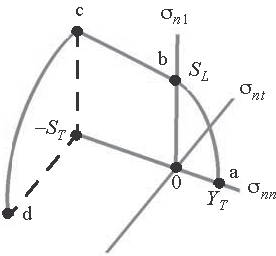
\includegraphics{Figure_9-4.pdf}}{\caption{Matrix failure locus in the $\sigma_{nn}$, $\sigma_{nt}$, and $\sigma_{n\textbf{1}}$ stress space for a unidirectional ply subject to plane stress. The failure locus is symmetric with respect to the $\sigma_{nn}$-$\sigma_{n\textbf{1}}$ plane and the $\sigma_{nn}$-$\sigma_{nt}$ plane.}\label{fig9.4}}

\begin{table}[!h]
\processtable{Stress components at selected points labeled in figure~\ref{fig9.4} \label{tab9.3}}{
\tabcolsep=8pt\begin{tabular}{@{}lccccc@{}}
\toprule
\colhead{Point} & \colhead{$\sigma_{n n}$} & \colhead{$\sigma_{n t}$} & \colhead{$\sigma_{n {\textbf{1}}}$} & \colhead{$\sigma_{{\textbf{22}}}$} & \colhead{$\sigma_{{\textbf{21}}}$} \\
\midrule
a &$Y_{T}$ & 0 & 0 & $Y_{T}$ & 0 \\
b &0 &0 &$S_{L}$& 0 &$S_{L}$ \\
c &$-S_{T}$& 0& $S_{L}\sqrt{1+2 p_{n t}^{(-)}}$ & $-S_{T}$ & $S_{L}\sqrt{1+2 p_{n t}^{(-)}}$ \\
d &$-S_{T}$ & $-Y_{C}\cos \alpha_{f} \sin \alpha_{f}$$^{\textrm{a}}$ & 0 & $-Y_{C}$ & 0 \\
\botrule
\end{tabular}}{${\textrm{a.}}$ $\cos \alpha_{f}=\left[2\left(1+p_{n t}^{(-)}\right)\right]^{-1/2}$}
\end{table}

The matrix failure locus shown in figure~\ref{fig9.4} is plotted in the $\sigma_{22}$-$\sigma_{21}$ stress plane in figure~\ref{fig9.5}.

\processfigure[!h]{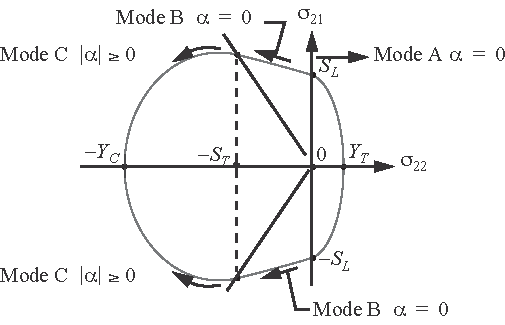
\includegraphics{Figure_9-5.pdf}}{\caption{Matrix failure modes for Puck's criterion in the $\sigma_{{\textbf{22}}}$-$\sigma_{{\textbf{21}}}$ stress plane for a unidirectional ply.}\label{fig9.5}}

In multidirectional laminates the intralaminar failure predictions are made by the analysis of strains and/or stresses in each lamina, with failure criteria evaluated in each lamina. A failure initiated in one lamina predicts the onset of damage, or first ply failure (FPF), that is usually not the ultimate failure of the laminate. It is insufficient to predict ultimate failure with the failure initiation criteria alone if the composite structure can accumulate damage before ultimate failure.

\clearpage

\section{Stresses in the principal material directions}\label{sec9.2}

The stresses in the \textit{k-th} ply, $k=1,2, \ldots, N p$, of the laminated wall are required to assess the strength of the ply. Starting from eq.~(\ref{eq8.27}) on page~\pageref{eq8.27} we have for the $k$-\textit{th} ply
\begin{align}\label{eq9.54}
\left[\begin{array}{@{}l@{}}\sigma_{11} \\\sigma_{22} \\\sigma_{12}\end{array}\right]^{(k)}=[Q]\left[\begin{array}{@{}l@{}}\varepsilon_{11} \\\varepsilon_{22} \\\gamma_{12}\end{array}\right]^{(k)},
\end{align}
where the reduced stiffness matrix is
\begin{align}\label{eq9.55}
[Q]=\left[\begin{array}{@{}ccc@{}}E_{1} /\left(1-v_{21} v_{12}\right) & \left(v_{12} E_{1}\right) /\left(1-v_{21} v_{12}\right) & 0 \\\left(v_{21} E_{2}\right) /\left(1-v_{21} v_{12}\right) & E_{2} /\left(1-v_{21} v_{12}\right) & 0 \\0 & 0 & G_{12}\end{array}\right].
\end{align}
The strains in the principal material directions are related to the strains in the beam coordinate directions by eq.~(\ref{eq8.29}), which is repeated below.
\begin{align}\label{eq9.56}
\left[\begin{array}{@{}l@{}}\varepsilon_{11} \\\varepsilon_{22} \\\gamma_{12}\end{array}\right]^{(k)}=\left[T_{\varepsilon 2}\left(\varphi_{k}\right)\right]\left[\begin{array}{@{}l@{}}\varepsilon_{s s} \\\varepsilon_{z z} \\\gamma_{z s}\end{array}\right]=\left[\begin{array}{@{}ccc@{}}n^{2} & m^{2} & m n \\m^{2} & n^{2} & -m n \\-2 m n & 2 m n & \left(-m^{2}+n^{2}\right)\end{array}\right]\left[\begin{array}{@{}l@{}}\varepsilon_{s s} \\\varepsilon_{z z} \\\gamma_{z s}\end{array}\right],
\end{align}
where $m=\cos \varphi_{k}$ and $n=\sin \varphi_{k}$. Substitute eq.~(\ref{eq9.56}) for the strains in eq.~(\ref{eq9.54}) to get
\begin{align}\label{eq9.57}
\left[\begin{array}{@{}l@{}}\sigma_{11} \\\sigma_{22} \\\sigma_{12}\end{array}\right]^{(k)}=[Q]\left[T_{\varepsilon 2}\left(\varphi_{k}\right)\right]\left[\begin{array}{@{}l@{}}\varepsilon_{s s} \\\varepsilon_{z z} \\\gamma_{z s}\end{array}\right].
\end{align}
The axial normal strain $\varepsilon_{z z}$ and the shear strain $\gamma_{s z}$ are determined from the material law, eq.~(\ref{eq8.45}) on page~\pageref{eq8.45};~i.e.,
\begin{align}\label{eq9.58}
\varepsilon_{z z}=\frac{1}{B}\left(n_{z}-b q\right) \quad \gamma_{s z}=\frac{1}{B}\left(a q-b n_{z}\right).
\end{align}
The normal strain $\varepsilon_{ss}$ is determined from the assumption $n_{s}=0$ in eq.~(\ref{eq8.35}) on page~\pageref{eq8.35}, which yields
\begin{align}\label{eq9.59}
\varepsilon_{s s}=-\left(A_{12}/A_{11}\right) \varepsilon_{z z}-\left(A_{16}/A_{11}\right) \gamma_{z s}.
\end{align}
With the strains $\varepsilon_{z z}$, $\gamma_{zs}$, and $\varepsilon_{ss}$ determined from eq.~(\ref{eq9.58}) and eq.~(\ref{eq9.59}), the stresses in the material principal directions in the \textit{k}-\textit{th} ply are obtained from eq.~(\ref{eq9.57})

\begin{example}[First ply failure envelope for the circular tube in example~\ref{ex8.3}] \label{ex9.1}
\hspace*{-2pt}The graphite-epoxy tube is subject to a prescribed axial force \textit{N} and torque $\textit{M}_z$ at its free end, and no other external loads. Thus, the only internal actions at each cross section are an axial force \textit{N} and a torque $\textit{M}_z$. The shear flow $q$ from eq.~(\ref{eq8.74}), and the normal stress resultant $n$ from eq.~(\ref{eq8.77}), at each cross section reduce to
\begin{equation}
q=M_{z} /\left(2 A_{c}\right) \quad n_{z}=(B/S) N. \label{eq9.1.a}\tag{a}
\end{equation}
From eq. (\textbf{\ref{eq9.1.f}}) in example~\ref{ex8.3} on page~\pageref{ex8.3} the function $\Phi(\theta)=0$, $0 \leq \theta<2 \pi$, so the torque does not contribute to the expression for the normal stress resultant. From example~\ref{ex8.3} we have the following data:
\begin{equation*}
S=4.99669 \textrm{ MN} \quad b=-1.22899 \quad B=39.1363 \textrm{ MN}/\mathrm{m} \quad a=3.9495 \quad A_{c}=0.00129717\,\mathrm{m}^{2}.
\end{equation*}
\vspace*{2pt}
\clearpage

\noindent Consider proportional loading and take
\begin{equation}
q/n_{z}=\tan \beta=\left[S /\left(2 A_{c} B\right)\right]\left(M_{z}/N\right). \label{eq9.1.b}\tag{b}
\end{equation}
For $N=\lambda \cos \beta$, the torque $M_{z}=\left(2 A_{c} B/S\right) \lambda \sin \beta=(0.02032\,\mathrm{m}) \lambda \sin \beta$. A radial ray that runs from the origin to the point of failure initiation in the plane of the axial force and torque is shown in figure~\ref{fig9.6}. Use Puck's criterion, eqs. (\ref{eq9.51}) to (\ref{eq9.53}), to determine which of the two unidrectional layers with angles $\varphi_{1}=-20^{\circ}$ and $\varphi_{2}=70^{\circ}$ fail first. That is, we find the minimum value of $\lambda>0$ for specified values of $\beta$, $0 \leq \beta \leq 2 \pi$ to assess first ply failure. The strengths of T300/5208 graphite/epoxy are listed in table~\ref{tab9.4}.

\processfigure{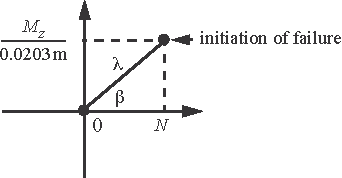
\includegraphics{Figure_9-6.pdf}}{\caption{A load ray in the plane of the axial force and torque}\label{fig9.6}}

\begin{table}[!h]
\processtable{Strength parameters for Puck's criterion: eqs. (\ref{eq9.51}) to (\ref{eq9.53}) \label{tab9.4}}{
\tabcolsep=10pt\begin{tabular}{@{}ll|ll@{}}
%\toprule
\hline
 & & & \\[-7pt]
$X_{T}$$^{\textrm{a}}$ & $1{,}454.72 \textrm{ MPa}$ ($\text { 211. ksi }$)  & $p_{n t}^{(-)}$  & 0.25\\[3pt]
$X_{C}$ & $1{,}454.72 \textrm{ MPa}$ ($\text { 211. ksi }$)  & $p_{n t}^{(+)}$  & 0.25\\[3pt]
$Y_{T}$$^{\textrm{a}}$  & $42.0559 \textrm{ MPa}$ ($6.1 \textrm{ ksi}$)  & $p_{n 1}^{(+)}$  & 0.25\\[3pt]
$Y_{C}$$^{\textrm{b}}$  & $246\textrm{ MPa}$  & $p_{n 1}^{(-)c}$  & 0.241725\\[3pt]
$s_{L}$$^{\textrm{a}}$  &  $95.1429 \textrm{ MPa}$ ($13.8 \textrm{ ksi}$) & $S_{T}$ & $98.4 \textrm{ MPa}$ \\[-7pt]
 & & & \\
\hline
%\botrule
\end{tabular}}{a. Nixon (1987). \\
b. Tsai (1992).\\
c. Equation (9.24).}\vspace*{-7pt}
\end{table}

The strains from the compliance law (\ref{eq9.58}) are
\begin{equation}
\varepsilon_{z z}=N/S-\left[b /\left(2 A_{c} B\right)\right] M_{z} \quad \gamma_{s z}=\left[a /\left(2 A_{c} B\right)\right] M_{z}-(b/S) N, \label{eq9.1.c}\tag{c}
\end{equation}
The normal strain $\varepsilon_{ss}$ in eq.~(\ref{eq9.59}) is evaluated from in-plane stiffness matrix is given by eq. (\textbf{\ref{eq9.1.a}}) of example~\ref{ex8.3}. The results for the laminate strains are
\begin{equation}
\left[\begin{array}{@{}l@{}}\varepsilon_{s s} \\\varepsilon_{z z} \\\gamma_{s z}\end{array}\right]=\left[\begin{array}{@{}cc@{}}1.99988 \times 10^{-7} & 12.0956 \times 10^{-6} \\-1.08262 \times 10^{-7} & -12.0956 \times 10^{6} \\2.45783 \times 10^{-7} & 38.8707 \times 10^{-6}\end{array}\right]\left[\begin{array}{@{}c@{}}N \\M_{z}\end{array}\right].\label{eq9.1.d}\tag{d}
\end{equation}
The reduced stiffness matrix is determined from the material property data listed in example~\ref{ex8.3} which yields the result
\begin{equation}
[Q]=\left[\begin{array}{@{}ccc@{}}148.461 & 4.2377 & 0 \\4.23777 & 11.152 & 0 \\0 & 0 & 6.4118\end{array}\right]\,\mathrm{GPa}. \label{eq9.1.e}\tag{e}
\end{equation}
The stresses in the principal directions of a ply are determined from eq.~(\ref{eq9.57}). For the $\varphi_{1}=-20^{\circ}$ ply, $m=0.939693$ and $n=-0.342020$ in eq.~(\ref{eq9.56}). The stresses in the principal material directions are
\begin{equation}
\left[\begin{array}{@{}l@{}}\sigma_{11} \\\sigma_{22} \\\sigma_{12}\end{array}\right]^{(1)}=[Q]\left[T_{\varepsilon 2}\left(-20^{\circ}\right)\right]\left[\begin{array}{@{}l@{}}\varepsilon_{s s} \\\varepsilon_{z z} \\\gamma_{s z}\end{array}\right]=\lambda\left[\begin{array}{@{}cc@{}}12{,}638.6 & -9{,}457.22 \\435.659 & 453.391 \\-2{,}477.65 & -5{,}905.5\end{array}\right]\left[\begin{array}{@{}l@{}}\cos \beta \\\sin \beta\end{array}\right]. \label{eq9.1.f}\tag{f}
\end{equation}
For the $\varphi_{2}=70^{\circ}$ ply, $m=0.342020$ and $n=0.939693$ in eq.~(\ref{eq9.56}). The stresses in the principal material directions~are
\begin{equation}
\left[\begin{array}{@{}l@{}}\sigma_{11} \\\sigma_{22} \\\sigma_{12}\end{array}\right]^{(2)}=[Q]\left[T_{\varepsilon 2}\left(70^{\circ}\right)\right]\left[\begin{array}{@{}l@{}}\varepsilon_{s s} \\\varepsilon_{z z} \\\gamma_{s z}\end{array}\right]=\lambda\left[\begin{array}{@{}cc@{}}1{,}367.92 & 9{,}347.22 \\975.989 & -453.391 \\2{,}477.65 & 5{,}905.5\end{array}\right]\left[\begin{array}{@{}l@{}}\cos \beta \\\sin \beta\end{array}\right]. \label{eq9.1.g}\tag{g}
\end{equation}

\vspace*{-1pc}

To illustrate the failure methodology we detail the first ply failure analysis for $\beta=30^{\circ}$ and $\beta=150^{\circ}$. The stress components in the material directions in each ply are listed in table~\ref{tab9.5}.

\begin{table}[!h]
\processtable{Stresses in the principal material directions in the ${\bf -20^{\circ}}$ ply and the ${\bf 70^{\circ}}$ ply for two different load rays \label{tab9.5}}{
\tabcolsep=10pt\begin{tabular}{@{}lllll@{}}
\toprule
 & \multicolumn{2}{l}{\colhead{$\boldsymbol{\beta}\ {\bf =30^{\circ}}$}} & \multicolumn{2}{l}{\colhead{$\boldsymbol{\beta}\ {\bf =150^{\circ}}$}} \\[-5pt]
 & \multicolumn{2}{l}{\hrulefill} & \multicolumn{2}{l}{\hrulefill} \\
\colhead{Stress} & \colhead{${\bf -20^{\circ}}$ ply} & \colhead{${\bf 70^{\circ}}$ ply} & \colhead{${\bf -20^{\circ}}$ ply} & \colhead{${\bf 70^{\circ}}$ ply} \\
\midrule
$\sigma_{11}$ & $\phantom{-}6{,}216.74 \lambda$ & $5{,}913.26 \lambda$ & $-15{,}674. \lambda$ & \phantom{$-$}$3{,}543.95 \lambda$ \\
$\sigma_{22}$ & $\phantom{-}603.987 \lambda$ & \phantom{5,}$618.536 \lambda$ & $-150.597 \lambda$ & $-1{,}071.93 \lambda$ \\
$\sigma_{21}$ & $-5{,}098.46 \lambda$ & $5{,}098.46 \lambda$ & $-807.041 \lambda$ & \phantom{$-$1,}$807.041 \lambda$ \\
\botrule
\end{tabular}}{}
\vspace*{-1pc}
\end{table}

\subsubsection{Computations for $\beta=30^{\circ}$.}\quad The stress component in the fiber direction $\sigma_{11}>0$ for both plies indicates a fiber tension mode of failure for $\lambda>0$. Since $\sigma_{11}$ is larger in the $-20^{\circ}$ ply it leads to a smaller value of  $\lambda$. From (\ref{eq9.35})
\begin{equation}
1=\frac{\left(6{,}216.741/\mathrm{m}^{2}\right) \lambda}{\left(1{,}454.72 \times 10^{6}\,\mathrm{N}/\mathrm{m}^{2}\right)}, \label{eq9.1.h}\tag{h}
\end{equation}
which is solved to find $\lambda=234{,}001\,\mathrm{N}$. In the $-20^{\circ}$ ply the stress components $\sigma_{22}>0$ and $\sigma_{21}<0$ which corresponds to the quadrant IV of the stress plane of figure~\ref{fig9.5}. Evaluation of the mode A failure criterion (\ref{eq9.51}) for the $-20^{\circ}$ ply leads to
\begin{equation}
1.58705 \times 10^{-6} \lambda+55.08999 \times 10^{-6} \sqrt{\lambda^{2}}=1. \label{eq9.1.i}\tag{i}
\end{equation}
The positive root of eq. (\textbf{\ref{eq9.1.i}}) is $\lambda=17{,}644.1\,\mathrm{N}$. In the $70^{\circ}$ ply the stresses $\sigma_{22}>0$ and $\sigma_{21}>0$, which corresponds to quadrant I of the stress plane. Evaluation of the mode A failure criterion (\ref{eq9.51}) for the $70^{\circ}$ ply leads to
\begin{equation}
1.62528 \times 10^{-6} \lambda+55.1611 \times 10^{-6} \sqrt{\lambda^{2}}=1. \label{eq9.1.j}\tag{j}
\end{equation}
The positive root of eq. (\textbf{\ref{eq9.1.j}}) is $\lambda=17{,}609.8\,\mathrm{N}$. The results of first ply failure analysis for $\beta=30^{\circ}$ is a matrix mode A failure in the $70^{\circ}$ ply at $\lambda=17{,}609.8\,\mathrm{N}$.

\subsubsection{Computations for $\beta=150^{\circ}$.}\quad The stress $\sigma_{11}<0$ in the $-20^{\circ}$ ply, and $\sigma_{11}>0$ in the $70^{\circ}$ ply for $\lambda>0$. The magnitude of $\sigma_{11}$ in the $-20^{\circ}$-ply exceeds the magnitude of $\sigma_{11}$ in the $70^{\circ}$-ply, so for fiber failure the $-20^{\circ}$-ply leads\vadjust{\vspace*{8pt}\pagebreak} to a smaller value of $\lambda$. Equating the fiber failure index in compression to equal one leads to
\begin{equation}
1=\frac{-\left(-15{,}674.1/\mathrm{m}^{2}\right) \lambda}{\left(1454.72 \times 10^{6}\,\mathrm{N}/\mathrm{m}^{2}\right)}, \label{eq9.1.k}\tag{k}
\end{equation}
which is solved to find $\lambda=92{,}811.4\,\mathrm{N}$.

In the $-20^{\circ}$-ply stresses $\sigma_{22}<0$, and $\sigma_{21}<0$, which means the matrix failure index is evaluated in quadrant III of the stress plane shown in figure~\ref{fig9.5}. To determine if the failure index is evaluated in the mode B or mode C sub-domain of quadrant III, we calculate the slope of the line representing the stress ratio $\sigma_{21}/ \sigma_{22}$ and compare it to the slope of the line dividing the mode B and mode C sub-domains. Let $m_{\sigma}$ denote the slope of the line determined by the stress ratio, and let $m_{b/c}$ denote the slope of the line dividing sub-domains in quadrant III. Refer to figure~\ref{fig9.5} to see that the stress coordinates $\sigma_{21}=-S_{L} \sqrt{1+2 p_{n t}^{(-)}}$ and $\sigma_{22}=-S_{T}$ define a point on the line subdividing mode B and mode C. The strength data is listed in table~\ref{tab9.4}. Numerical evaluation of the slopes\break yields
\begin{equation}
m_{\sigma}=\frac{-807.041 \lambda}{(-150.597 \lambda)}=5.359 \quad m_{b/c}=\frac{\left(-S_{L}\sqrt{1+2 p_{n t}^{(-)}}\right)}{-S_{T}}=1.184. \label{eq9.1.l}\tag{l}
\end{equation}
Since $m_{b/c}<m_{\sigma}<\infty$, the matrix failure index is evaluated in the mode B sub-domain of quadrant~III. Set the failure index in mode B (\ref{eq9.52}) equal to one to get the quadratic equation
\begin{equation}
\left(-7.65227 \times 10^{-7}+7.19512 \times 10^{-11} \lambda\right) \lambda=1. \label{eq9.1.m}\tag{m}
\end{equation}
The positive root of eq. (\textbf{\ref{eq9.1.m}}) is $\lambda=123{,}329.\,\mathrm{N}$.

In the $70^{\circ}$-ply the matrix stresses $\sigma_{22}<0$ and $\sigma_{21}>0$, so the matrix failure index is computed in quadrant II of the stress plane. To determine if the failure is a mode B or mode C, we again determine the slopes $m_{\sigma}$ and $m_{b/c}$ in quadrant~II. The numerical results for the slopes are
\begin{equation}
m_{\sigma}=\frac{807.041 \lambda}{-1{,}071.93 \lambda}=-0.752 \quad m_{b/c}=\frac{\left(S_{L}\sqrt{1+2 p_{n t}^{(-)}}\right)}{-S_{T}}=-1.184. \label{eq9.1.n}\tag{n}
\end{equation}
Since $m_{b/c}<m_{\sigma}<0$, the failure index is compute for mode C in quadrant II. Set the failure index in mode C (\ref{eq9.53}) equal to one to get
\begin{equation}
6.9994 \times 10^{-6} \lambda=1. \label{eq9.1.o}\tag{o}
\end{equation}
Hence, for the matrix mode C in the $70^{\circ}$ ply $\lambda=142{,}869\,\mathrm{N}$. For $\beta=150^{\circ}$ the minimum value of $\lambda$ is $92{,}811.4\,\mathrm{N}$, which corresponds to a fiber compression mode in the $-20^{\circ}$ ply.

The following table lists first ply failure results for selected values of $\beta$.

\begin{table}[!h]
\processtable{First ply failure data for selected load rays \label{tab9.6}}{
\tabcolsep=9pt\begin{tabular}{@{}lllll@{}}
\toprule
\colhead{$\beta$, degrees} & \colhead{$\lambda, \textrm{ N}$} & \colhead{Axial force $N, \textrm{ kN}$} & \colhead{Torque $M_{\textbf{\textit{z}}}$, N-m} & \colhead{Mode of failure} \\
\midrule
0 & 27{,}936.9 &  \phantom{$-0$}27.94 & \phantom{$-00$}0 & $\phantom{-}70^{\circ}$ ply matrix mode A \\
30 &  17{,}609.8 &  \phantom{$-0$}15.25 & \phantom{$-$}178.9& $\phantom{-}70^{\circ}$ ply matrix mode A \\
35 &  16{,}658.1 &  \phantom{$-0$}13.65& \phantom{$-$}194.2& $-20^{\circ}$ ply matrix mode A\\
90 &  15{,}625.6 &  \phantom{$-00$}0 &  \phantom{$-$}317.5 &  $-20^{\circ}$ ply matrix mode A\\
135 &  39{,}199.9 &  $\phantom{0}-$27.72 &  \phantom{$-$}563.2 &  $-20^{\circ}$ ply matrix mode A\\
140 &  50{,}399. &  $\phantom{0}-$38.61 &  \phantom{$-$}658.2 &  $-20^{\circ}$ ply matrix mode B\\
145 &  71{,}295.8 &  $\phantom{0}-$58.40 &  \phantom{$-$}831.0 &  $-20^{\circ}$ ply matrix mode B\\
150 &  92{,}811.4 &  $\phantom{0}-$80.38 &  \phantom{$-$}943.0 &  $-20^{\circ}$ ply fiber compression\\
155 &  94{,}149.1 &  $\phantom{0}-$85.33 &  \phantom{$-$}808.5 &  $-20^{\circ}$ ply fiber compression\\
160 &  96{,}269.3 &  $\phantom{0}-$90.46 &  \phantom{$-$}669.1 &  $-20^{\circ}$ ply fiber compression\\
165 &  99{,}260.1 &  $\phantom{0}-$95.88 &  \phantom{$-$}522.0 &  $-20^{\circ}$ ply fiber compression\\
170 &  71.408. &  $-$101.7 &  \phantom{$-$}364.3 &  $-20^{\circ}$ ply matrix mode B\\
180 &  40{,}067.3 &  $\phantom{0}-$51.14 &  \phantom{$-00$}0 &  $-20^{\circ}$ ply matrix mode B\\
210 &  19{,}203.1 &  $\phantom{0}-$17.91 &  $-$210.1 &  $-20^{\circ}$ ply matrix mode B\\
215 &  17{,}992.2 &  $\phantom{0}-$15.73 &  $-$223.8 &  $-70^{\circ}$ ply matrix mode B\\
245 &  14{,}868.6 &  $\phantom{00}-$6.352 &  $-$276.8 &  $-70^{\circ}$ ply matrix mode B\\
250 &  14{,}814. &  $\phantom{00}-$5.085 &  $-$283.9 &  $-70^{\circ}$ ply matrix mode A\\
270 &  15{,}625.6 &  \phantom{$-00$}0 &  $-$310.1 &  $-70^{\circ}$ ply matrix mode A\\
335 &  38{,}849.7 &  \phantom{$-0$}33.53 &  $-$317.8 &  $-70^{\circ}$ ply matrix mode A\\
355 &  30{,}944.9 &  \phantom{$-0$}34.02 &  $\phantom{0}-$60.49 &  $\phantom{-}70^{\circ}$ ply matrix mode A\\
\botrule
\end{tabular}}{}
\end{table}

Note that the majority of first ply failures are matrix modes A and B. For $150^{\circ} \leq \beta \leq 165^{\circ}$ the mode of failure is fiber compression in the $-20^{\circ}$ ply. The first ply failure locus is plotted in figure~\ref{fig9.7}.
\end{example}

\processfigure{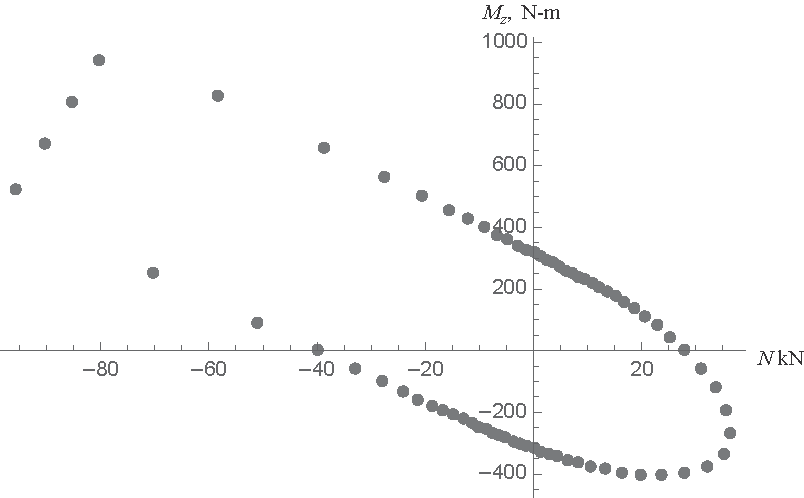
\includegraphics{Figure_9-7.pdf}}{\caption{First ply failure locus for the graphite epoxy circular tube subject to an axial force and a torque.}\label{fig9.7}}

\clearpage

\begin{thebibliography}{}\label{sec9.3}
\bibitem{} Dowlng, N. E. \textit{\textbf{Mechanical Behavior of Materials}}. Englewood Cliffs, NJ: Prentice Hall, Inc., 1993.

\bibitem{} Herakovich, Carl T. \textit{\textbf{Mechanics of Fibrous Composites}}. New York: John Wiley \& Sons, Inc., 1998.

\bibitem{} Nixon, M. W. ``Extension-Twist Coupling of Composite Circular Tubes with Application to Tilt Rotor Blade Design.'' In \textit{Proceedings of the 28th Structures, Structural Dynamics, and Materials Conference} (Monterey, CA). Reston, VA: American Institute of Aeronautics and Astronautics, 1987.

\bibitem{} Puck, A., and H. Schürmann. ``Failure Analysis of FRP Laminates by Means of Physically Based Phenomenological Models.'' \textit{\textbf{Composites Science and Technology}} 58 (1998):1045--1067.

\bibitem{} Puck, A., J. Kopp, and M. Knops., ``Guidelines for the Determination of the Parameters in Puck's Action Plane Strength Criterion.'' \textit{\textbf{Composites Science and Technology}}, 62 (2002): 371--378.

\bibitem{} Soden, P. D., A. S. Kaddour, and M. J. Hinton. ``Recommendations for Designers and Researchers Resulting from the World Wide Failure Exercise.'' \textit{\textbf{Composites Science and Technology}}, 64 (2004): 589--601.

\bibitem{} Tsai, S. W. \textit{\textbf{Theory of Composites Design}}. Dayton, OH: THINK COMPOSITES, a Division of ILT Corporation, 1992.
\end{thebibliography}

\cleardoublepage


\end{document}